%!TEX root =presentation.tex
\section[network adjoint]{Adjoint method applied to PDE networks} % (fold)
\label{sec:adjoint_method_applied_to_pde_networks}


\begin{frame}[t]
\frametitle{PDE with control}

Modify formulation to include

\begin{itemize}
    \item state vector $\state\in\mathbb{R}^{\nlinks \ntime}$
    \item control vector $\control\in\mathbb{R}^{\ncontrols \ntime}$
    \begin{itemize}
        \item $\tuple{\condiscrete{\cind_{\jn}^{1}}{\tind}}{\condiscrete{\cind_{\jn}^{\ncontrols_{\jn}}}{\tind}}\in\mathbb{R}^{\ncontrols_{\jn}}$ modifies Riemann problem at $\jn$ for time $\tind$.
        \begin{eqnarray*}
\RS_{\jn}: & \mathbb{R}^{\ninc_{\jn}+\nout_{\jn}}\times\mathbb{R}^{\ncontrols_{\jn}} & \rightarrow\mathbb{R}^{\ninc_{\jn}+\nout_{\jn}}\\
 & \left(\juncstate{\jn}{\tind},\junccon{\jn}{\tind}\right) & \mapsto\RS_{\jn}\left(\juncstate{\jn}{\tind},\junccon{\jn}{\tind}\right)=\junctrace{\jn}{\tind}
\end{eqnarray*}
        \item $\ncontrols$ are the number of control parameters at each time-step.
    \end{itemize}
\end{itemize}

Updated discrete state equations:

\begin{eqnarray}
\syseq_{\link}^{\tind}\left(\state,\control\right)= & \discrete{\link}{\tind}-\discrete{\link}{\tind-1} & +\dfrac{\Delta t}{\Delta x}\left(\god_{\jdown{\link}}\left(\juncstate{\jdown{\link}}{\tind},\junccon{\jdown{\link}}{\tind-1}\right)\right)_{\link}\nonumber \\
 &  & -\dfrac{\Delta t}{\Delta x}\left(\god_{\jup{\link}}\left(\juncstate{\jup{\link}}{\tind},\junccon{\jup{\link}}{\tind-1}\right)\right)_{\link}\label{eq:syseq-god}
\end{eqnarray}

\end{frame}

\begin{frame}[t]\frametitle{Optimization problem}
    

\begin{block}{Optimization Problem}
\begin{eqnarray}
\underset{\control}{\min} & \cost\left(\state,\control\right)\nonumber \\
\text{subject to:} & \sys\left(\state,\control\right)=0\label{eq:op-problem}
\end{eqnarray}
\end{block}

\begin{block}{Review: adjoint method}
\begin{equation}
d_{\control}\cost\left(\nominal{\state},\nominal{\control}\right)=\lambda^{T}\Hu+\Ju\label{eq:adjoint-grad}
\end{equation}
where
\begin{equation}
\Hx^{T}\lambda=-\Jx^{T}\label{eq:adjoint}
\end{equation}


\end{block}


\end{frame}

\begin{frame}


Assume initial $\control$ and state $\state$ where $\sys\left(\state, \control\right) = 0$.
\begin{block}{What needs to be computed for adjoint method?}
\begin{itemize}
    \item $\Jx$, $\Ju$: Problem specific, no sparsity assumptions.
    \item $\Hx$, $\Hu$: can analyze properties of PDE networks and Godunov scheme to:
    \begin{itemize}
        \item derive partial derivative expressions
        \item understand sparsity
    \end{itemize}
\end{itemize}
\end{block}

\end{frame}

\begin{frame}[t]\frametitle{Partial derivates of state equations}

\begin{block}{$\Hx$}
By chain rule:
\begin{align*}
\pfrac{\syseq_{\link}^{\tind}}{\discrete jl}=\pfrac{\discrete{\link}{\tind}}{\discrete jl}-\pfrac{\discrete{\link}{\tind-1}}{\discrete jl}+ \\
\frac{\Delta t}{L_{i}}\left(\pfrac{}{\discrete jl}\left(\god_{\jdown{\link}}\left(\juncstate{\jdown{\link}}{\tind-1},\junccon{\jdown{\link}}{\tind-1}\right)\right)_{\link}-\pfrac{}{\discrete jl}\left(\god_{\jup{\link}}\left(\juncstate{\jup{\link}}{\tind-1},\junccon{\jup{\link}}{\tind-1}\right)\right)_{\link}\right)\label{eq:dhdugod}
\end{align*}

\begin{itemize}
    \item Only require knowledge of partial derivatives on Godunov fluxes $\god$.
    \item $\pfrac{}{\discrete jl}\left(\god_{\jdown{\link}}\left(\juncstate{\jdown{\link}}{\tind-1},\junccon{\jdown{\link}}{\tind-1}\right)\right)_{\link} = 0$ unless $l = k - 1$.
    \item $\pfrac{}{\discrete jl}\left(\god_{\jdown{\link}}\left(\juncstate{\jdown{\link}}{\tind-1},\junccon{\jdown{\link}}{\tind-1}\right)\right)_{\link}= 0$ unless $j$ is downstream of $i$.
    \item Similar results for $\jup{i}$.
\end{itemize}
\end{block}
\end{frame}

\begin{frame}[t]\frametitle{Partial derivates of state equations}

\begin{block}{$\Hx$}
\begin{itemize}
    \item Only require knowledge of partial derivatives on Godunov fluxes $\god$.
    \item $\pfrac{}{\discrete jl}\left(\god_{\jdown{\link}}\left(\juncstate{\jdown{\link}}{\tind-1},\junccon{\jdown{\link}}{\tind-1}\right)\right)_{\link} = 0$ unless $l = k - 1$.
    \item $\pfrac{}{\discrete jl}\left(\god_{\jdown{\link}}\left(\juncstate{\jdown{\link}}{\tind-1},\junccon{\jdown{\link}}{\tind-1}\right)\right)_{\link}= 0$ unless $j$ is downstream of $i$.
    \item Similar results for $\jup{i}$.
\end{itemize}
Thus each partial term is zero unless variable is from previous time-step and adjacent to constraint link (or $i=j$ and $l=k$.
\end{block}
\end{frame}

\begin{frame}

\begin{figure}
\subfloat[\label{fig:partial-ordering}Ordering of the partial derivative terms.
Constraints and state variables are clustered first by time, and then
by cell index.]{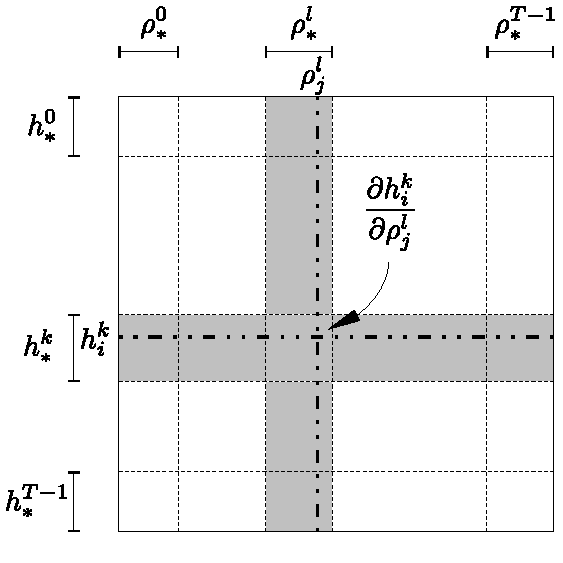
\includegraphics[width=0.45\columnwidth]{../figs-gen/dstate}

}\texttt{\hfill{}}\subfloat[\label{fig:sparsity-diagram}Sparsity structure of the $\Hx$ matrix.
Besides the diagonal blocks, which are identity matrices, blocks where
$l\neq\tind-1$ are zero.]{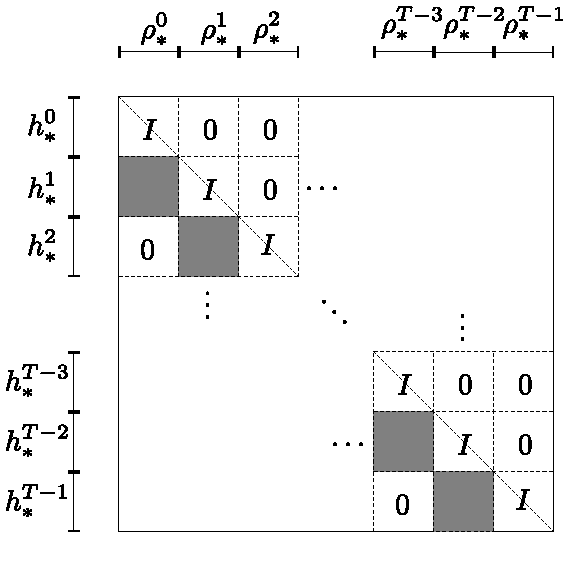
\includegraphics[width=0.45\columnwidth]{../figs-gen/sparsity-two}

\texttt{}

}

\caption{Structure of the $\Hx$ matrix.}


\end{figure}
\end{frame}

\begin{frame}[t]\frametitle{Partial derivates of state equations}

\begin{block}{$\Hu$}
By chain rule:
\begin{equation}
\pfrac{\syseq_{\link}^{\tind}}{\condiscrete jl}=\frac{\Delta t}{L_{i}}\left(\pfrac{}{\condiscrete jl}\left(\god_{\jdown{\link}}\left(\juncstate{\jdown{\link}}{\tind-1},\junccon{\jdown{\link}}{\tind-1}\right)\right)_{\link}-\pfrac{}{\condiscrete jl}\left(\god_{\jup{\link}}\left(\juncstate{\jup{\link}}{\tind-1},\junccon{\jup{\link}}{\tind-1}\right)\right)_{\link}\right)\label{eqdhdvgod}
\end{equation}
Similar arguments to $\Hx$ give us that each partial term above is zero unless control variable $\condiscrete jl$ is from same time-step and in $\tuple{\condiscrete{\cind_{\jup{\link}}^{1}}{\tind}}{\condiscrete{\cind_{\jup{\link}}^{\ncontrols_{\jup{\link}}}}{\tind}}$ or $\tuple{\condiscrete{\cind_{\jdown{\link}}^{1}}{\tind}}{\condiscrete{\cind_{\jdown{\link}}^{\ncontrols_{\jdown{\link}}}}{\tind}}$.
\end{block}
\end{frame}

% \begin{frame}[t]\frametitle{Example for linear flux function}

% \begin{example}
% On board...
% \end{example}

% \end{frame}


% section adjoint_method_applied_to_pde_networks (end)